\section{Introduction to Mathematical Morphology}
\label{sec:introduction_to_mathematical_morphology}



\setcounter{subsection}{1}
\subsection{Erosion and Dilation}
% question 2 image:
\textbf{Question 1} \textit{Define erosion and dilatation from an ensemblist point of view and an functional point of view. Give some properties related to these operators.}

\TODO{}


\textbf{Question 2} \textit{Operate in a binary image and a greyscale image with the MatLab commands imerode and imdilate. What are the effects on binary and grayscale images? Justify. Try with different structuring elements (different shapes, different sizes).}

In the figure below, the eroded and dilated images can be seen plotted next to the original image for each structuring element with the following shapes in order: rectangle, disk, diamond and line. \TODO{Mention something about the different quality of output for these? Which one is best?}

\vfill

\begin{figure}[H]
    \centering
    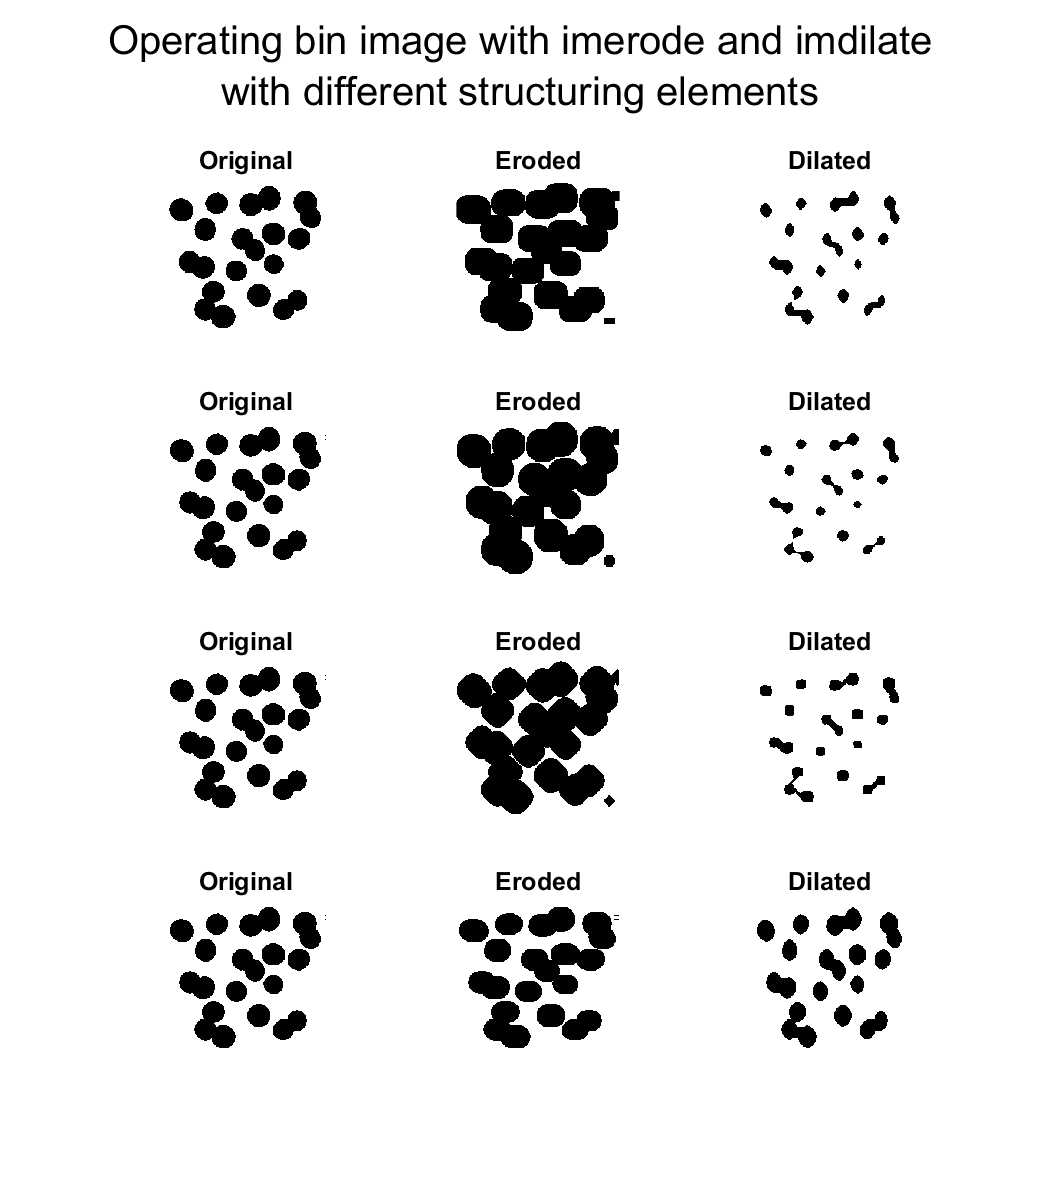
\includegraphics[width=0.75\linewidth]{Doc/Graphics/Part2/part2_Question2.png}
\end{figure}


\newpage
\textbf{Question 3} \textit{Extract internal and external edges of a binary image, and the morphological gradian.}
\begin{figure}[h]
    \centering
    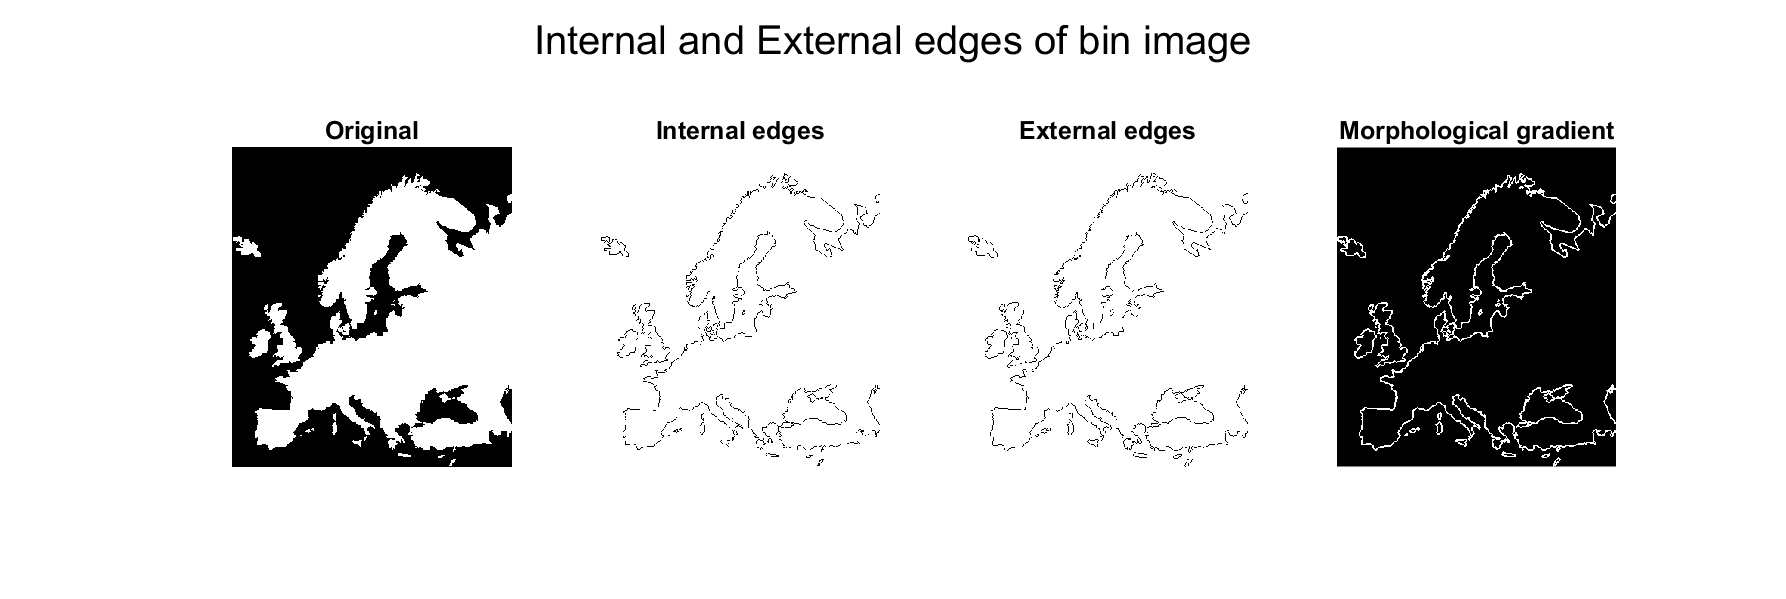
\includegraphics[width=1\linewidth]{Doc/Graphics/Part2/Part2_Question3.png}
\end{figure}


\textbf{Question 4} \textit{As an exercise, write an algorithm that show, in the map of Europe, the distance of each pixel w.r.t. the sea.}
\begin{figure}[h]
    \centering
    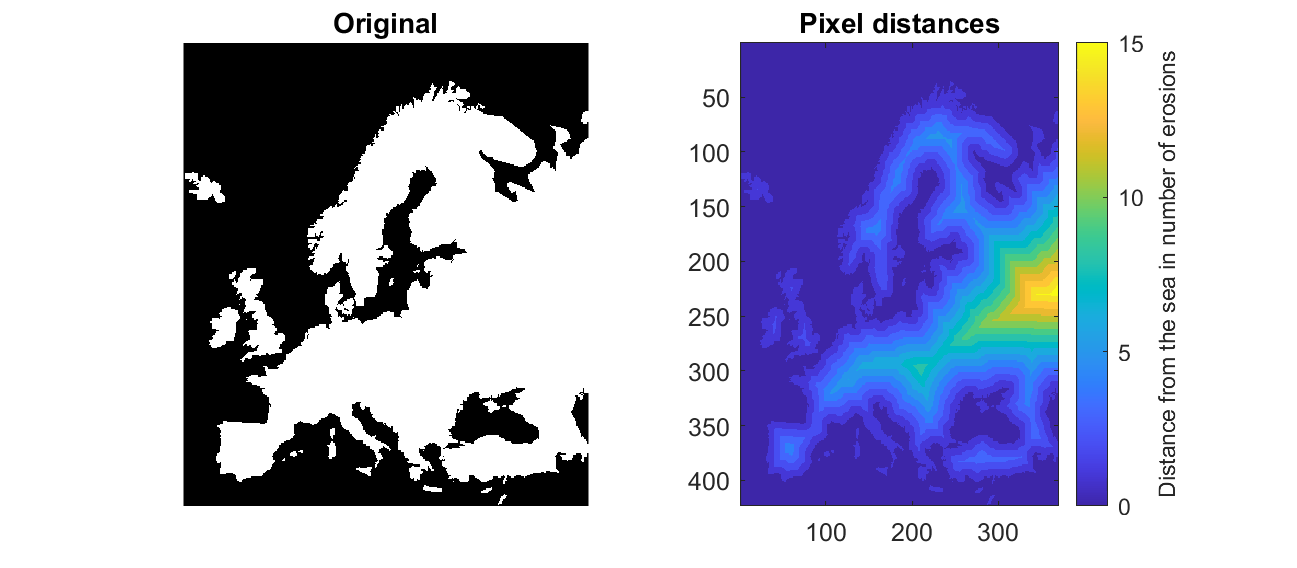
\includegraphics[width=0.75\linewidth]{Doc/Graphics/Part2/part2_Question4.png}
\end{figure}



\textbf{Question 5} \textit{Find an algorithm that detect rectangular objects of ’image2.jpg’.}

\begin{figure}[H]
    \centering
    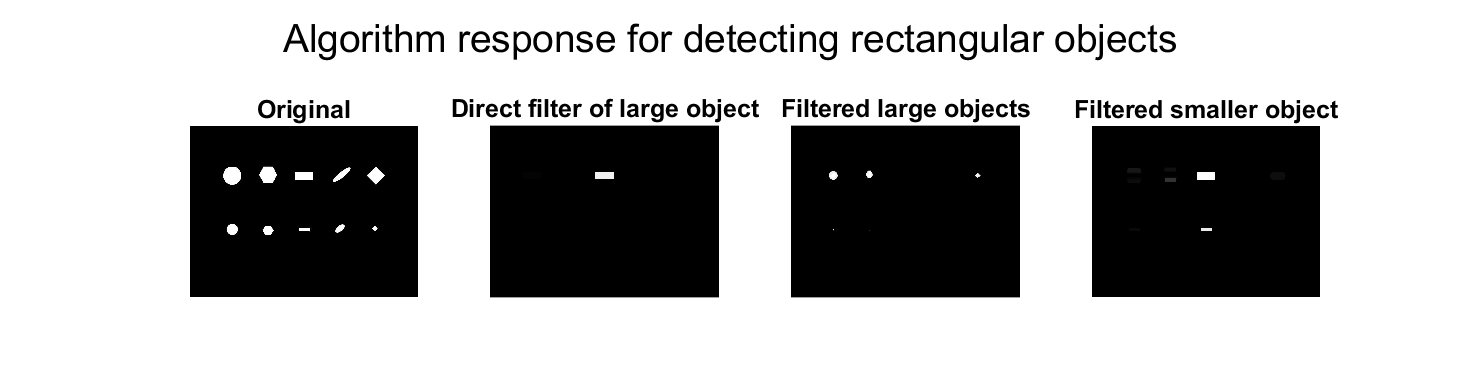
\includegraphics[width=\linewidth]{Doc/Graphics/Part2/Part2_Q5.png}
\end{figure}


\subsection{Morphological Filtering}
\subsubsection{Filters}
\textbf{Question 6} \textit{Define the two morphological filters called opening and closing. What are the effects on a binary image sur as ’image1.jpg’ (use the commands imopen and imclose)?}

\begin{itemize}
    \item \textbf{Opening filter:}
    \TODO{some text}

    \item  \textbf{Closing filter:}
    \TODO{some text}
    
\end{itemize}

\begin{figure}[H]
    \centering
    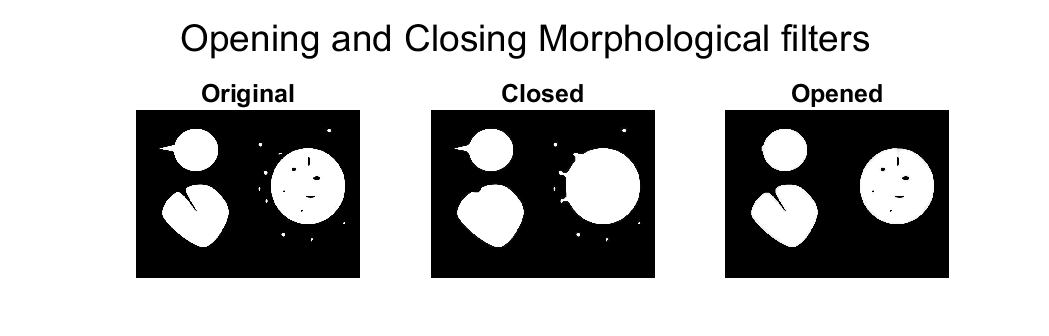
\includegraphics[width=0.75\linewidth]{Doc/Graphics/Part2/part2_Q6.png}
\end{figure}

\vfill
\subsubsection{Form Detection}
\textbf{Question 7} \textit{The objective being to recognize some forms on images, find a simple algorithm to operate form detection}

See Question 5, can easily be modified for different shapes, i.e. circle, diamond etc.


\textbf{Question 8} \textit{Apply a salt-and-pepper noise: what’s happen with your previous algorithm?}

The algorithm breaks and does not function at all due to the noise in the picture. See below:

\begin{figure}[H]
    \centering
    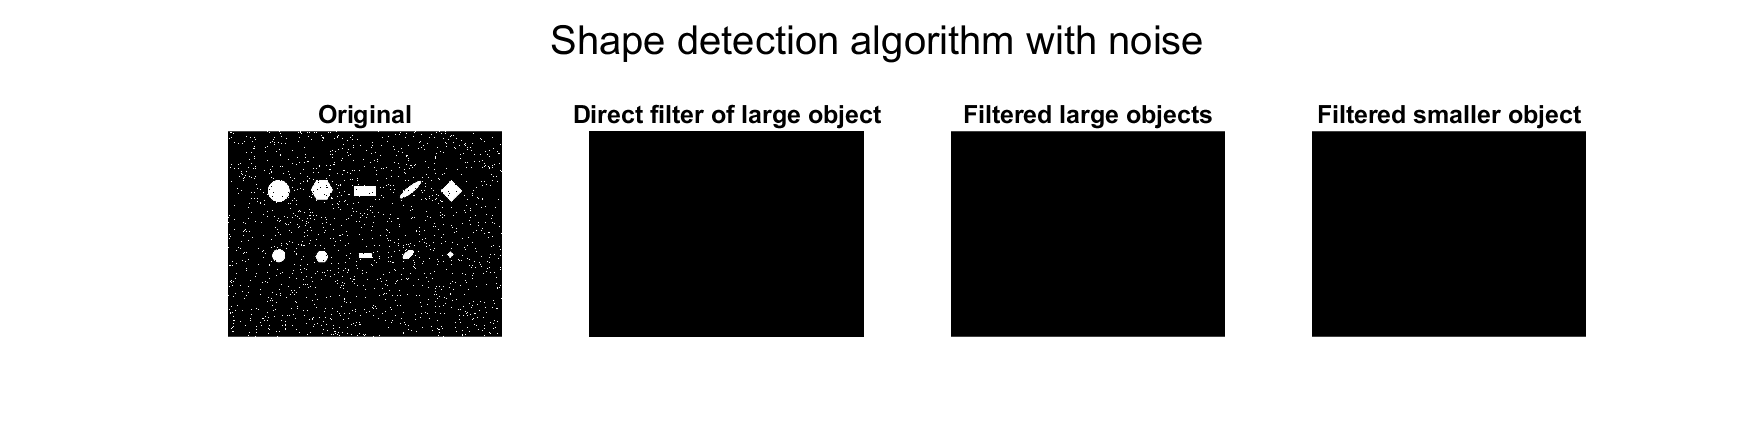
\includegraphics[width=\linewidth]{Doc/Graphics/Part2/part2_Q8.png}
\end{figure}



\newpage
\subsubsection{Denoising}
\textbf{Question 9} \textit{Use the image Nebuleuse.jpg and apply a salt-and-pepper noise. De-noise the image by filtering.}

\begin{figure}[H]
    \centering
    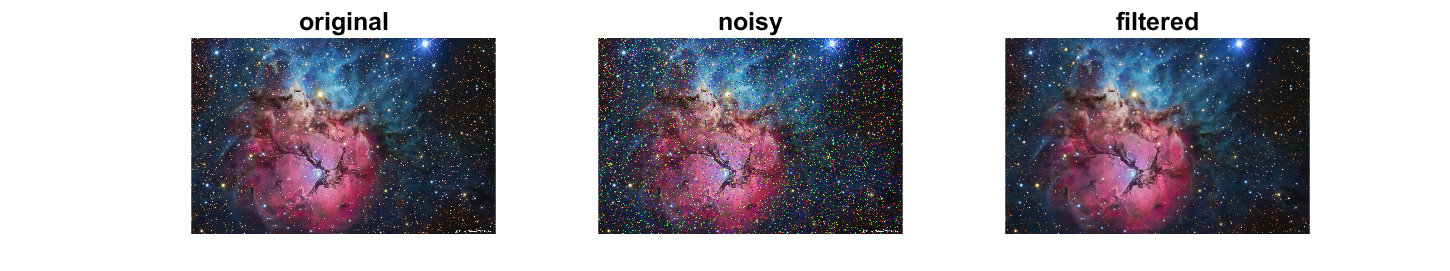
\includegraphics[width=\linewidth]{Doc/Graphics/Part2/part2_Q9.png}
\end{figure}


\textbf{Question 10} \textit{Apply the same process to the ’Spain Beach’ image to isolate the beach itself.}

\begin{figure}[H]
    \centering
    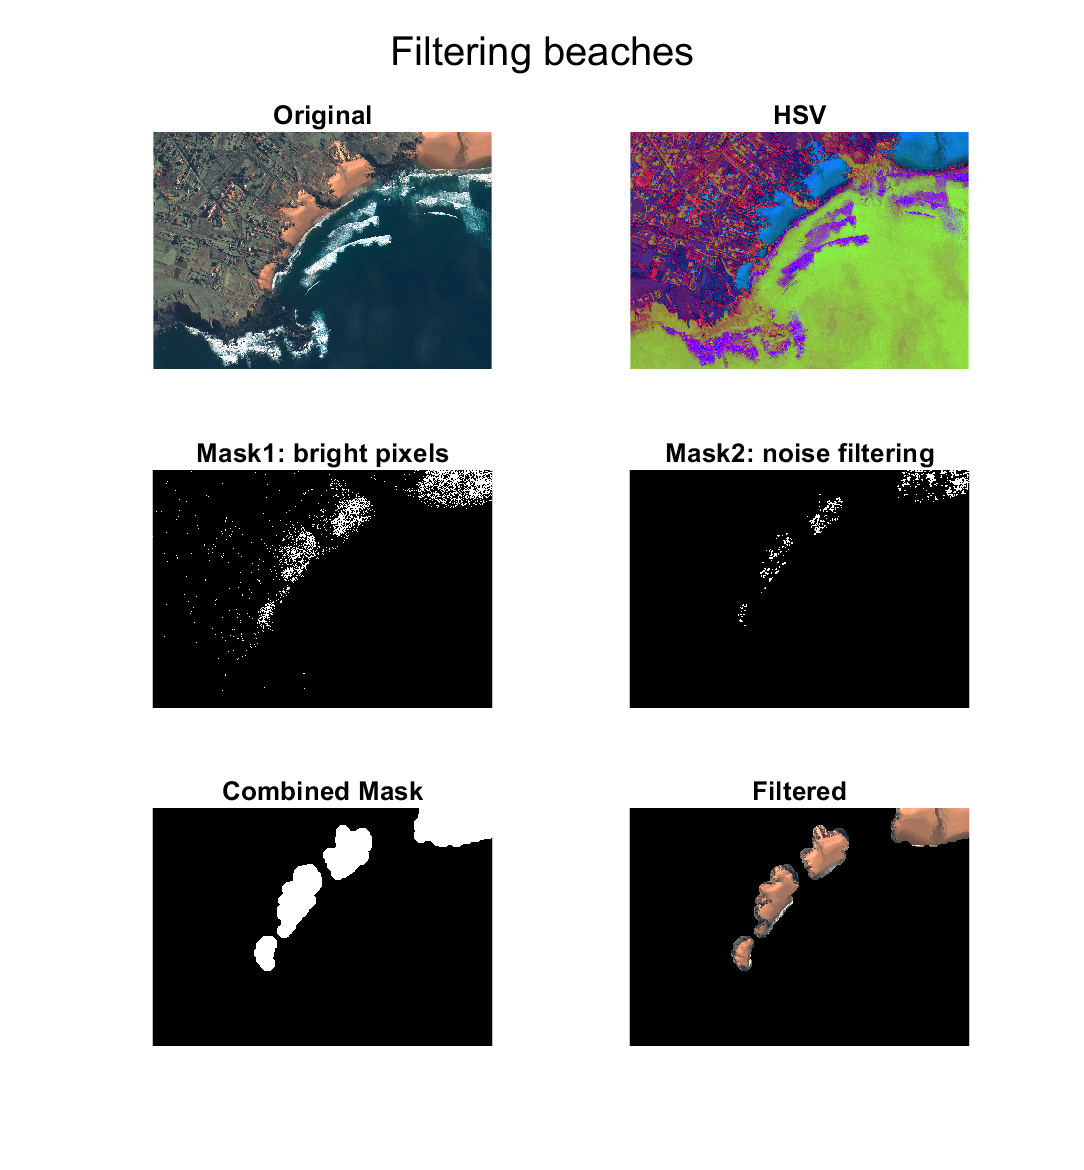
\includegraphics[width=0.75\linewidth]{Doc/Graphics/Part2/part2_Q10.png}
\end{figure}




\newpage
\subsubsection{Top-Hat \& Black-Hat Filters}
\textbf{Question 11} \textit{Define op-hat and black-hat process in a 1D function: what is the associated process?}

\textcolor{red}{TODO Write shit here}


\textbf{Question 12} \textit{Define and operate top-hat and black-hat on a greyscale image. What do you observe?}

\textcolor{red}{TODO Write shit here}


\subsection{Morphological Skeletonization \& Segmentation}
\subsubsection{Skeletonization Process}
\textbf{Question 13} \textit{Write and operate a Skeletonization on the diplodocus.}

\begin{figure}[H]
    \centering
    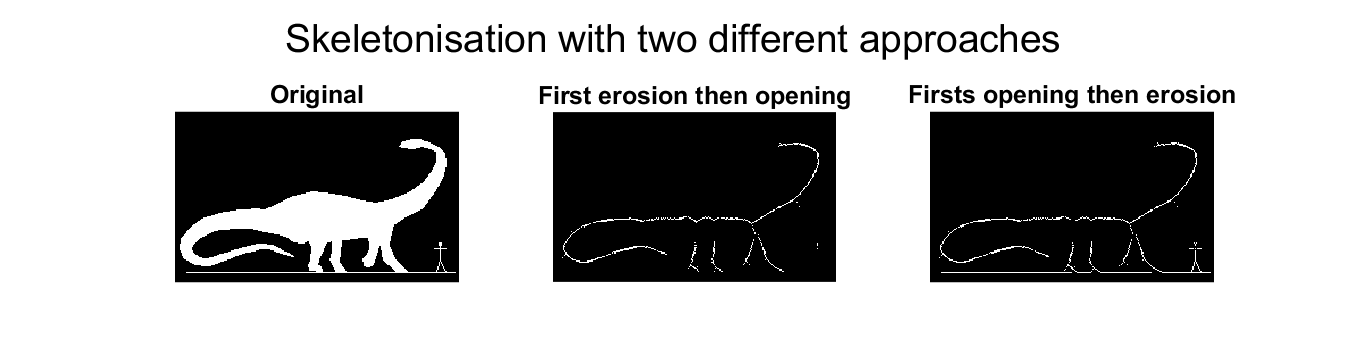
\includegraphics[width=\linewidth]{Doc/Graphics/Part2/part2_Q13.png}
\end{figure}


\textbf{Question 14} \textit{Based on skelittization, find an algorithm that operate a segmentation in a binary image. Apply on ’image1.jpg’.}

\begin{figure}[H]
    \centering
    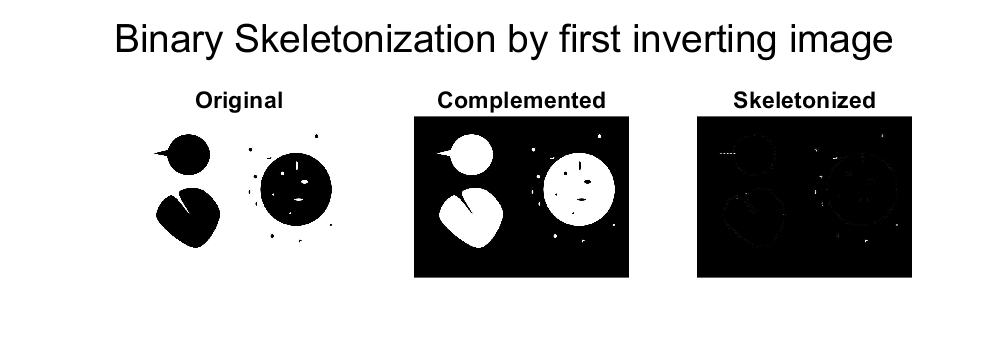
\includegraphics[width=\linewidth]{Doc/Graphics/Part2/part2_Q14.png}
\end{figure}



\newpage
\subsubsection{Image Segmentation}
\textbf{Question 15} \textit{Find a Skeletonization algorithm and operate on the Blood Cells image.}

\TODO{Write about why this does not work really well for the "real" image of the blood cells, even if we "binarise" it... Write about what steps we could take to maybe make it work?}

\begin{figure}[H]
    \centering
    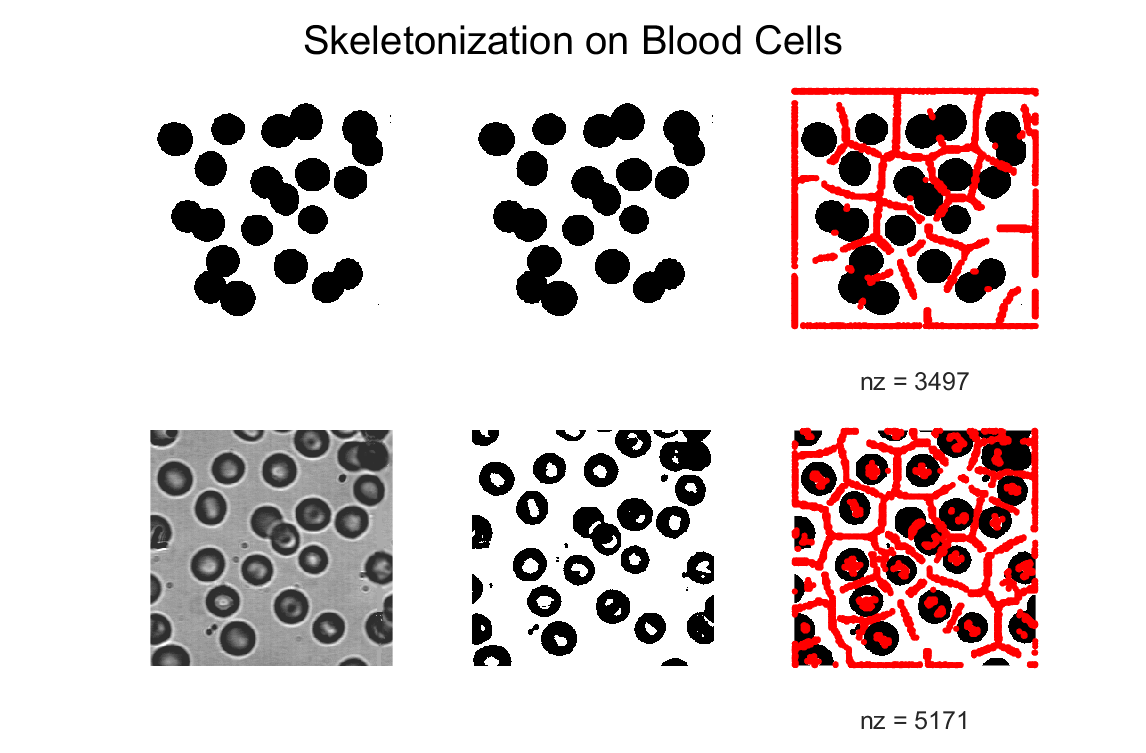
\includegraphics[width=\linewidth]{Doc/Graphics/Part2/part2_Q15.png}
\end{figure}
